Experiments were done mostly with the ShapeNet dataset \cite{shapenet}, which is a large dataset of 3D models. A random set of either 1024 or 2048 point clouds were sampled and then upscaled to double or quadruple the number of points.

At this stage only qualitative results are shown, and quantitative results will be shown in the final paper. 
Further, comparisons with other non-deep learning based methods, as well control studies comparing our method of placing with an octree and then smoothing to randomly placing points and then smoothing, will be done in the final paper.

\subsection{Evaluation Metrics}

We will eventually evaluate our model using the Chamfer distance and Hausdroff distance as they are common metrics used in point cloud upsampling, and try to compare to other parameter free works as well as deep learning based methods.
The Chamfer distance is a measure of how different 2 shapes are and is defined as the following:

$$ C(P, Q) = \dfrac{1}{|P|} \sum\limits_{p \in P} \min_{q \in Q} \norm{p - q}^2 +  \dfrac{1}{|Q|} \sum\limits_{q \in Q} \min_{p \in P} \norm{p - q}^2 \label{eq:chamfer}$$

The Hausdroff distance is a measure of how similar 2 sets are. It is defined as the following:

$$ H(A, B) = \max(h(A, B), h(B, A))\label{eq:hausdroff}$$

Where:

$$h(A, B) = \max_{a \in A} \min_{b \in B} \norm{a - b}$$

\subsection{Preliminary Results}

In this subsection we qualitatively compare results with octree upsampling only, and no smoothing, as well as both octree sampling and bilateral smoothing.

\begin{figure*}[!ht]
	\centering
	\begin{subfigure}{0.3\textwidth}
		\centering
		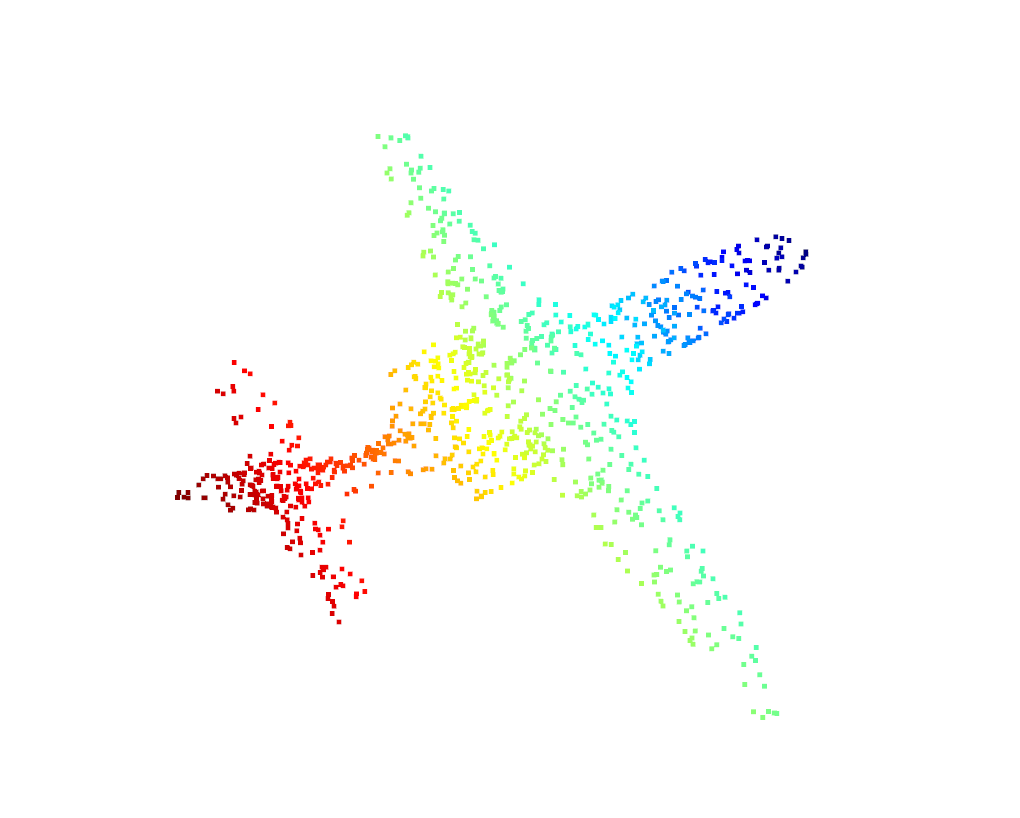
\includegraphics[width=\textwidth]{1024_no_upsampling.png}
		\caption{Original point cloud, with 1024 points}
	\end{subfigure}
	\begin{subfigure}{0.3\textwidth}
		\centering
		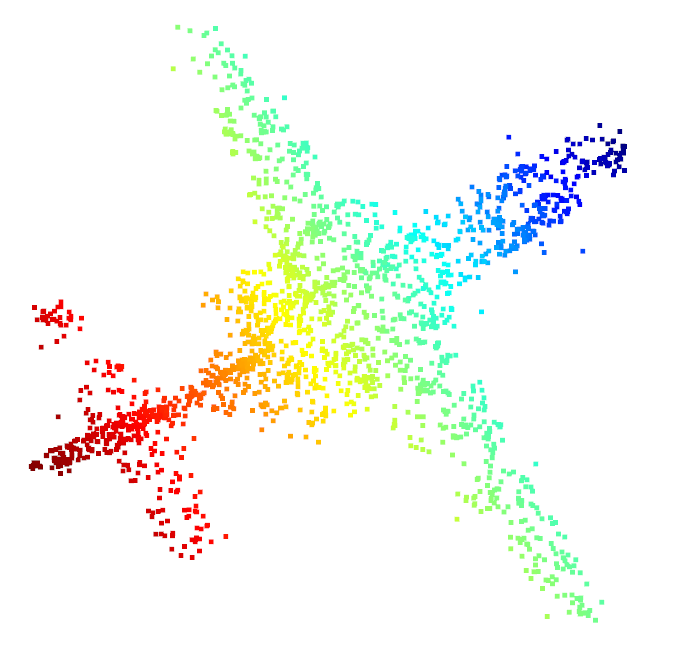
\includegraphics[width=0.65\textwidth]{./2048_octree_no_smoothing.png}
		\caption{Upsampled point cloud, with 2048 points using only octree and no smoothing}
	\end{subfigure}
	\begin{subfigure}{0.3\textwidth}
		\centering
		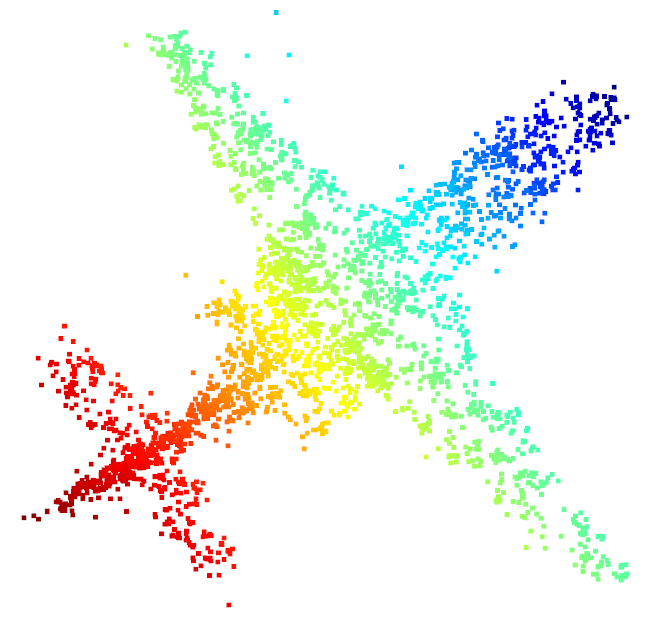
\includegraphics[width=0.65\textwidth]{./4096_octree_no_smoothing.png}
		\caption{Upsampled point cloud, with 4096 points using only octree and no smoothing}
	\end{subfigure}	
	\caption{A comparison of the original point cloud and the upsampled point cloud using only octree and no smoothing.}
	\label{fig:no_smoothing}
\end{figure*}

\begin{figure*}[!ht]
	\centering
	\begin{subfigure}{0.3\textwidth}
		\centering
		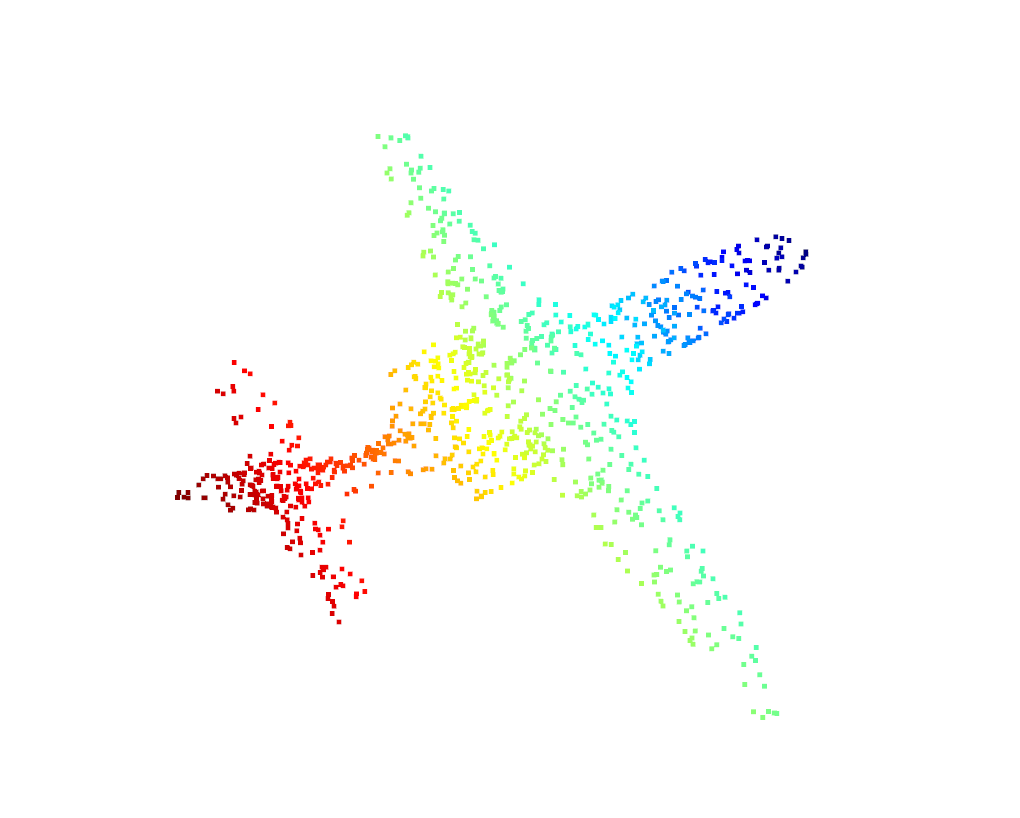
\includegraphics[width=\textwidth]{1024_no_upsampling.png}
		\caption{Original point cloud, with 1024 points}
	\end{subfigure}
	\begin{subfigure}{0.3\textwidth}
		\centering
		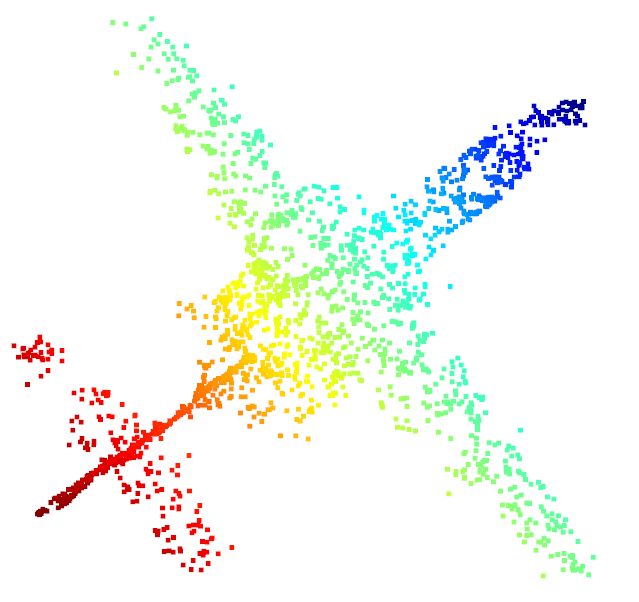
\includegraphics[width=0.65\textwidth]{./2048_octree_bilateral}
		\caption{Upsampled point cloud, with 2048 points using only octree and bilateral smoothing}
	\end{subfigure}
	\begin{subfigure}{0.3\textwidth}
		\centering
		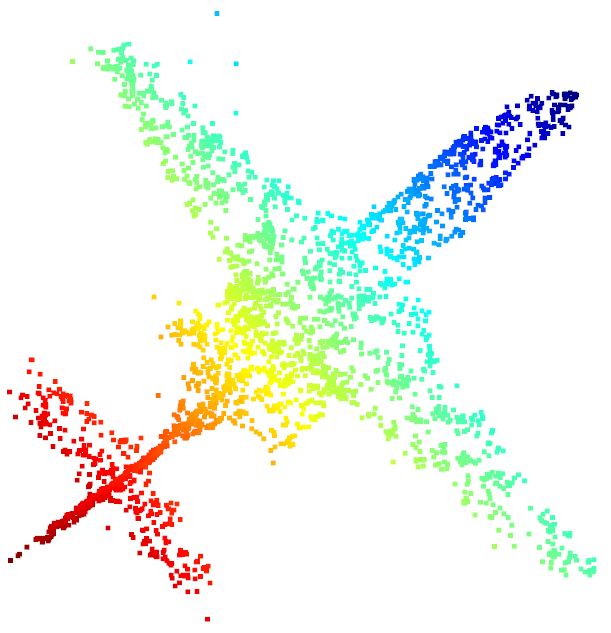
\includegraphics[width=0.65\textwidth]{./4096_octree_bilateral.png}
		\caption{Upsampled point cloud, with 4096 points using only octree and no smoothing}
	\end{subfigure}	
	\caption{A comparison of the original point cloud and the upsampled point cloud using only octree and bilateral smoothing.}
	\label{fig:no_smoothing}
\end{figure*}


